\documentclass[12pt,letterpaper]{article}
\usepackage{graphicx,textcomp}
\usepackage{natbib}
\usepackage{setspace}
\usepackage{fullpage}
\usepackage{color}
\usepackage[reqno]{amsmath}
\usepackage{amsthm}
\usepackage{fancyvrb}
\usepackage{amssymb,enumerate}
\usepackage[all]{xy}
\usepackage{endnotes}
\usepackage{lscape}
\newtheorem{com}{Comment}
\usepackage{float}
\usepackage{hyperref}
\newtheorem{lem} {Lemma}
\newtheorem{prop}{Proposition}
\newtheorem{thm}{Theorem}
\newtheorem{defn}{Definition}
\newtheorem{cor}{Corollary}
\newtheorem{obs}{Observation}
\usepackage[compact]{titlesec}
\usepackage{dcolumn}
\usepackage{tikz}
\usetikzlibrary{arrows}
\usepackage{multirow}
\usepackage{xcolor}
\newcolumntype{.}{D{.}{.}{-1}}
\newcolumntype{d}[1]{D{.}{.}{#1}}
\definecolor{light-gray}{gray}{0.65}
\usepackage{url}
\usepackage{listings}
\usepackage{color}

\definecolor{codegreen}{rgb}{0,0.6,0}
\definecolor{codegray}{rgb}{0.5,0.5,0.5}
\definecolor{codepurple}{rgb}{0.58,0,0.82}
\definecolor{backcolour}{rgb}{0.95,0.95,0.92}

\lstdefinestyle{mystyle}{
	backgroundcolor=\color{backcolour},   
	commentstyle=\color{codegreen},
	keywordstyle=\color{magenta},
	numberstyle=\tiny\color{codegray},
	stringstyle=\color{codepurple},
	basicstyle=\footnotesize,
	breakatwhitespace=false,         
	breaklines=true,                 
	captionpos=b,                    
	keepspaces=true,                 
	numbers=left,                    
	numbersep=5pt,                  
	showspaces=false,                
	showstringspaces=false,
	showtabs=false,                  
	tabsize=2
}
\lstset{style=mystyle}
\newcommand{\Sref}[1]{Section~\ref{#1}}
\newtheorem{hyp}{Hypothesis}

\title{\textbf{Replication of:} Lee, C. (2019). China’s Energy Diplomacy: Does Chinese Foreign Policy Favor Oil-Producing Countries? Foreign Policy Analysis, 15(4), 570–588. https://doi.org/10.1093/fpa/orz011

}
\date{Due: March 31, 2024}
\author{Applied Stats II \\ \vspace{\baselineskip}
	\textbf{Maiia Skrypnyk 23371609}}

\begin{document}
	\maketitle

\section{Replication Results }

\textbf{Loading the data:}
\lstinputlisting[language=R, firstline=11, lastline=14]{MSChina_energy_Lee_replicate.R} 


\textbf{Table 1:}

\lstinputlisting[language=R, firstline=18, lastline=60]{MSChina_energy_Lee_replicate.R} 


\begin{figure}[H]
    \centering
    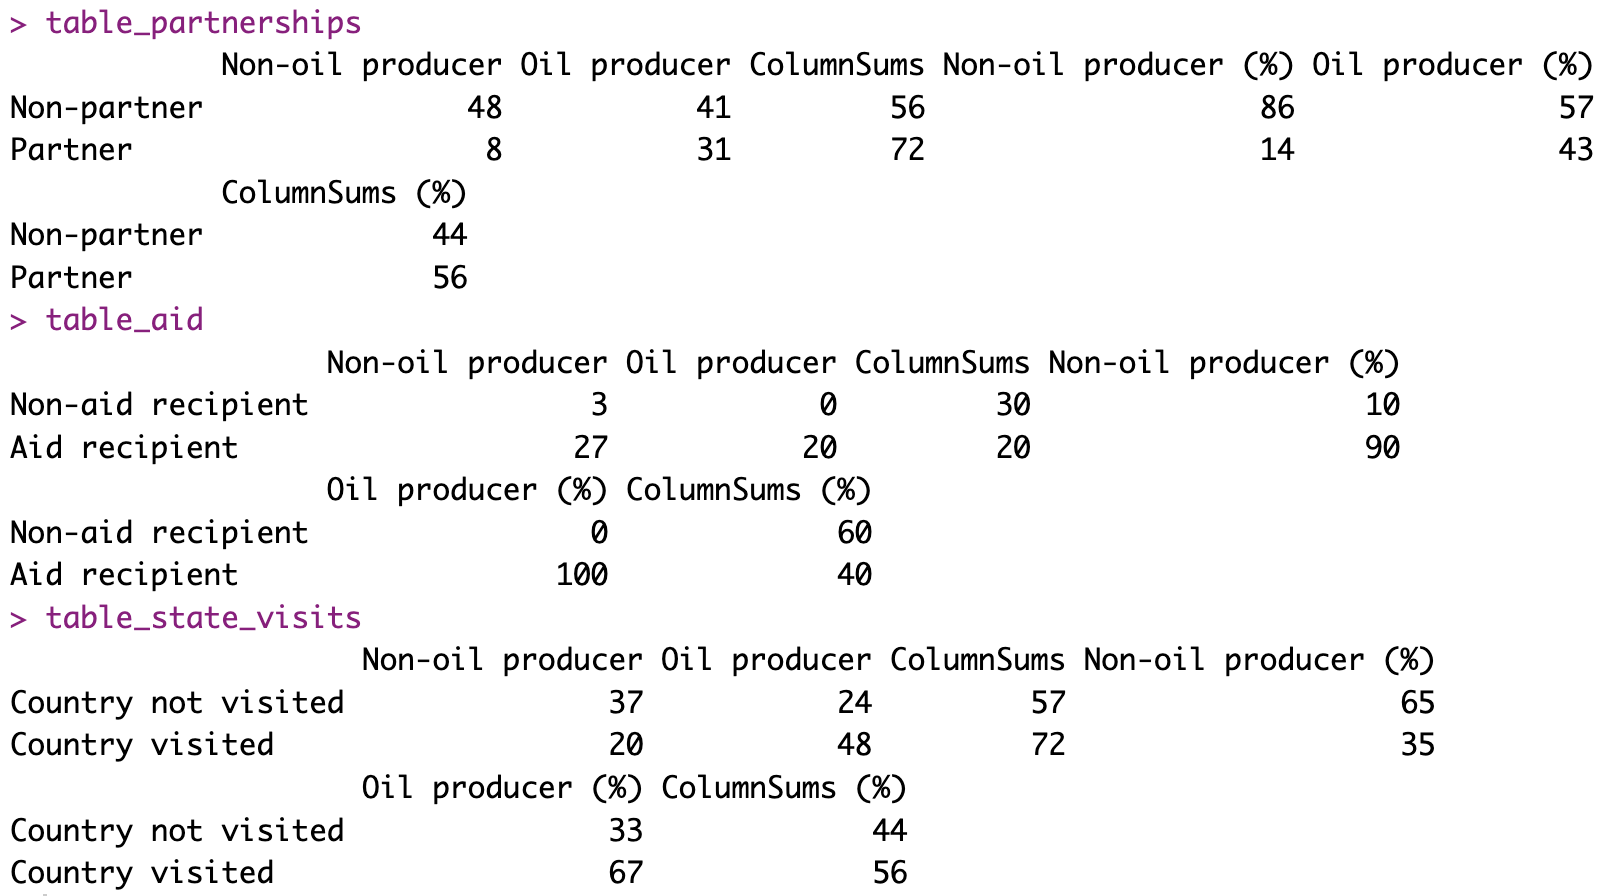
\includegraphics[width=0.9\linewidth]{table1r.png}
\end{figure}

The original Table 1 from the article for reference:

\begin{figure}[H]
    \centering
    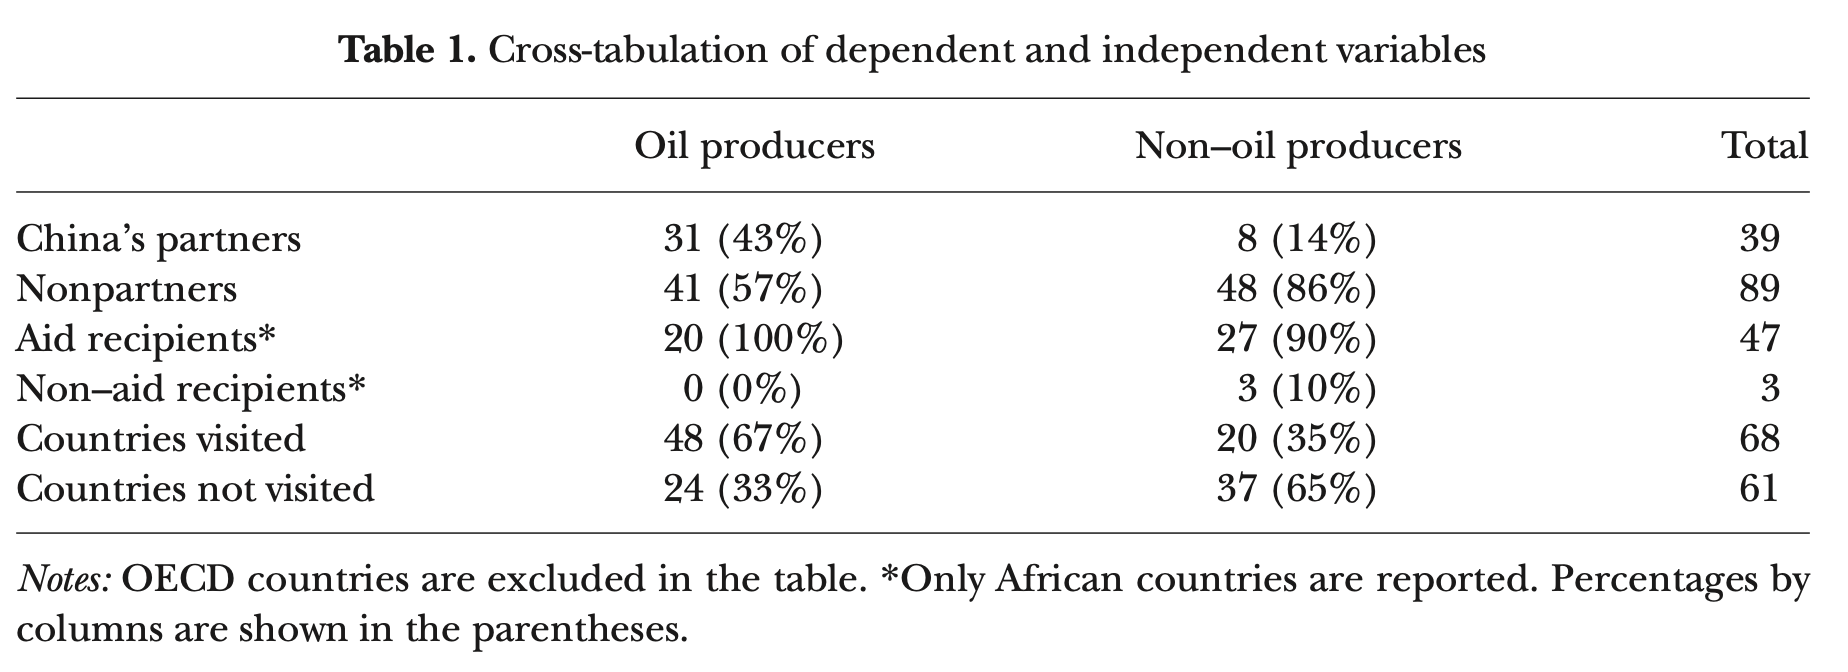
\includegraphics[width=0.75\linewidth]{table1.png}
\end{figure}

\textbf{Table 2:}

\lstinputlisting[language=R, firstline=62, lastline=92]{MSChina_energy_Lee_replicate.R} 

\begin{figure}[H]
    \centering
    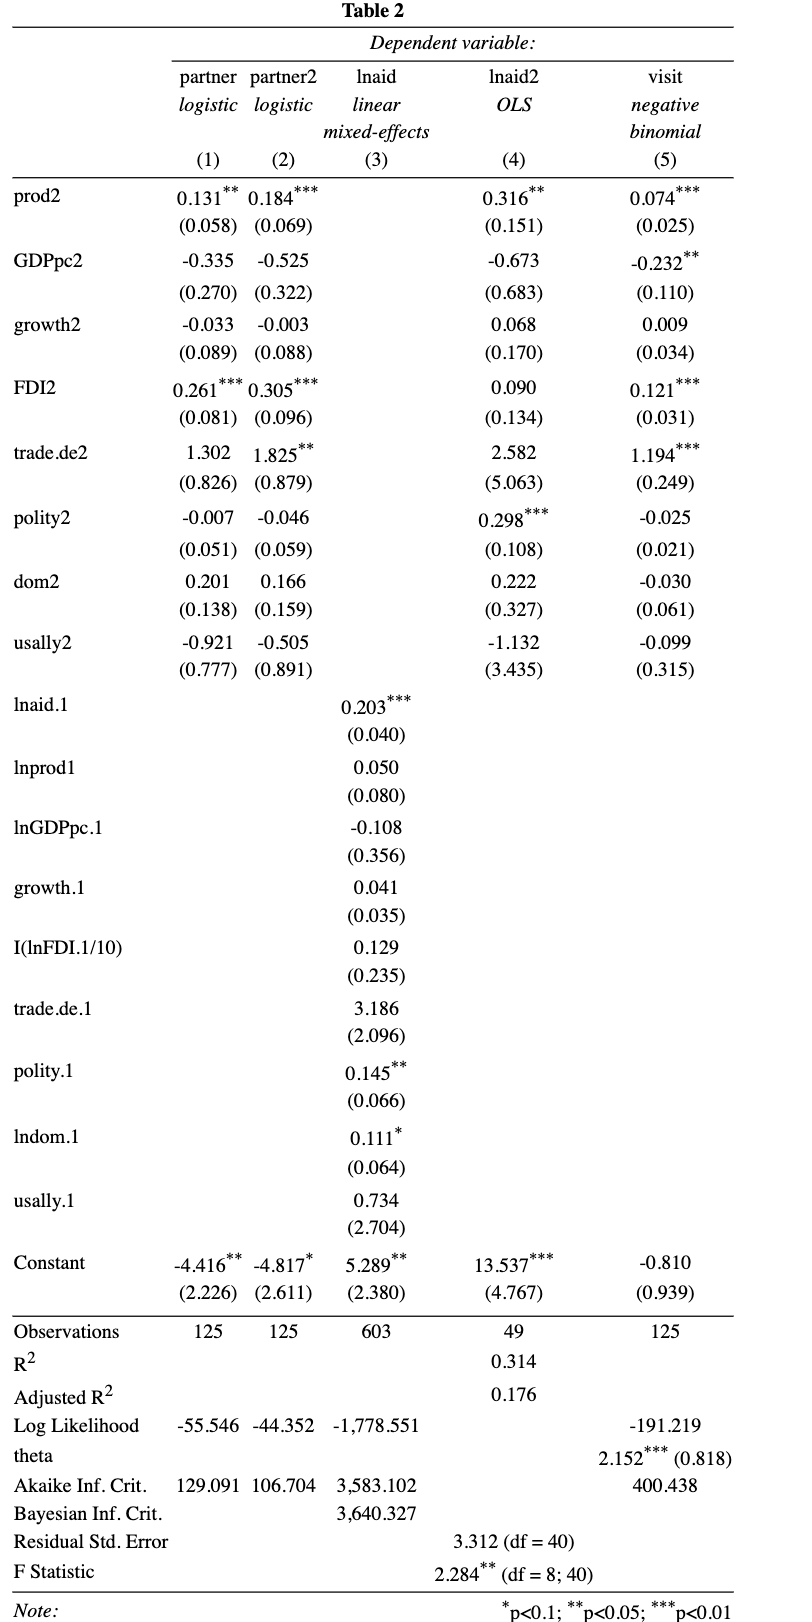
\includegraphics[width=0.6\linewidth]{table2r.png}
\end{figure}

\newpage 
\textbf{Table 3:}

\lstinputlisting[language=R, firstline=94, lastline=128]{MSChina_energy_Lee_replicate.R} 

\begin{figure}[H]
    \centering
    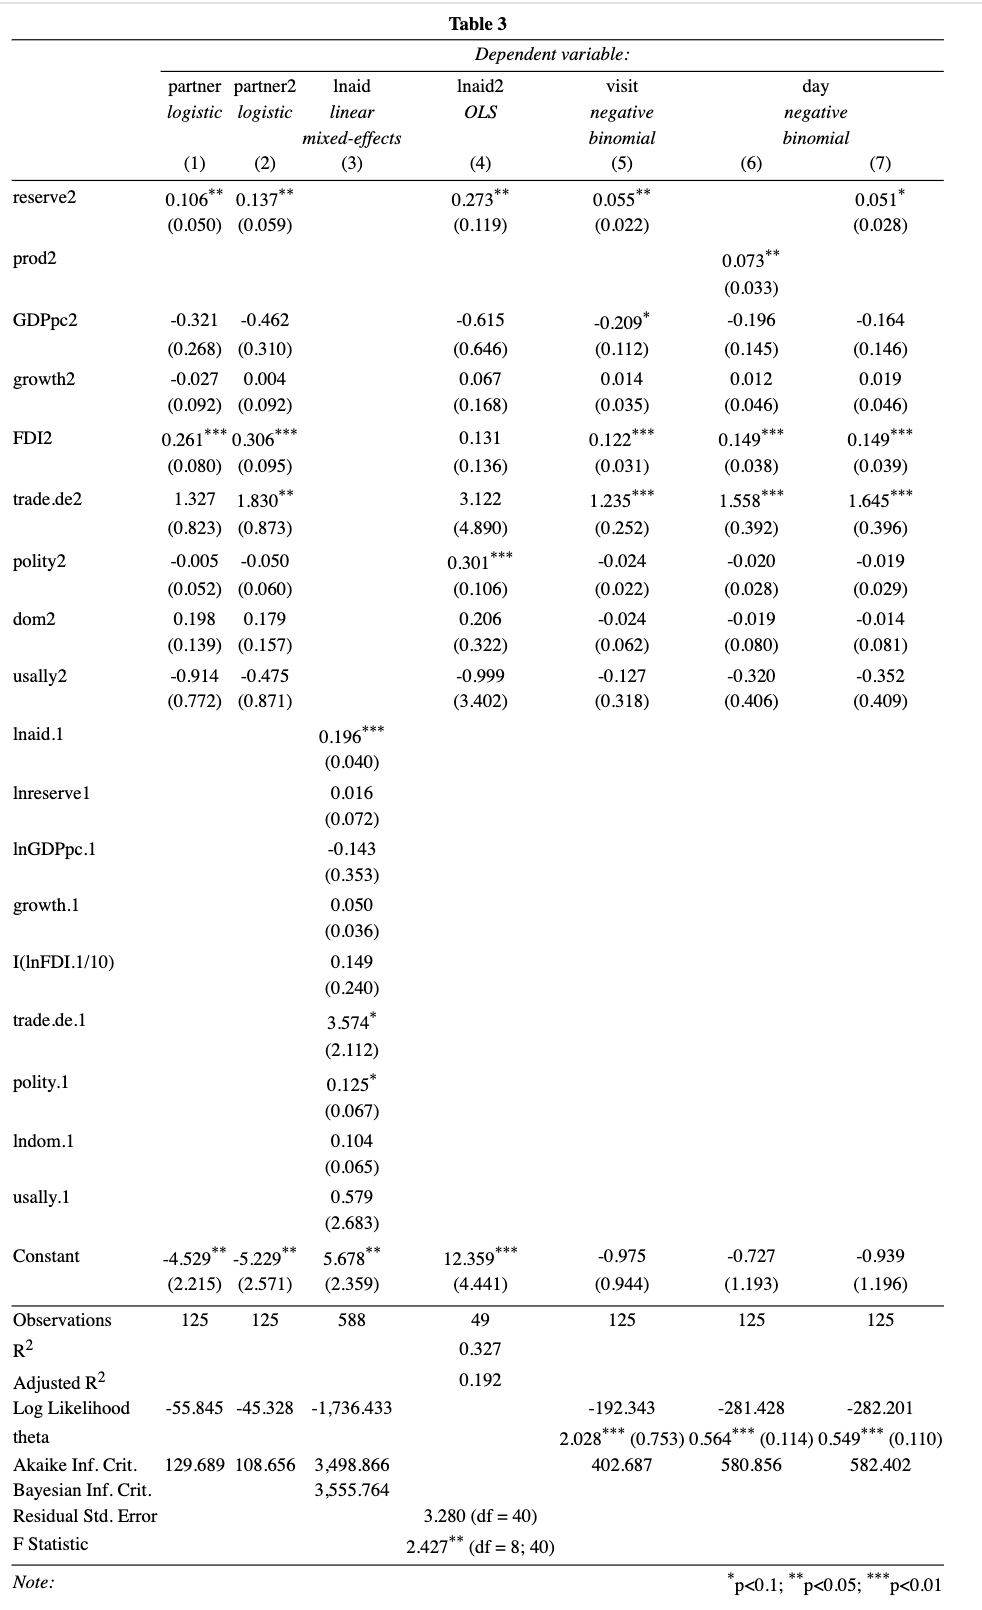
\includegraphics[width=0.8\linewidth]{table3r.png}
\end{figure}

\textbf{Figure 1:}
\lstinputlisting[language=R, firstline=130, lastline=155]{MSChina_energy_Lee_replicate.R} 

\begin{figure}[H]
    \centering
    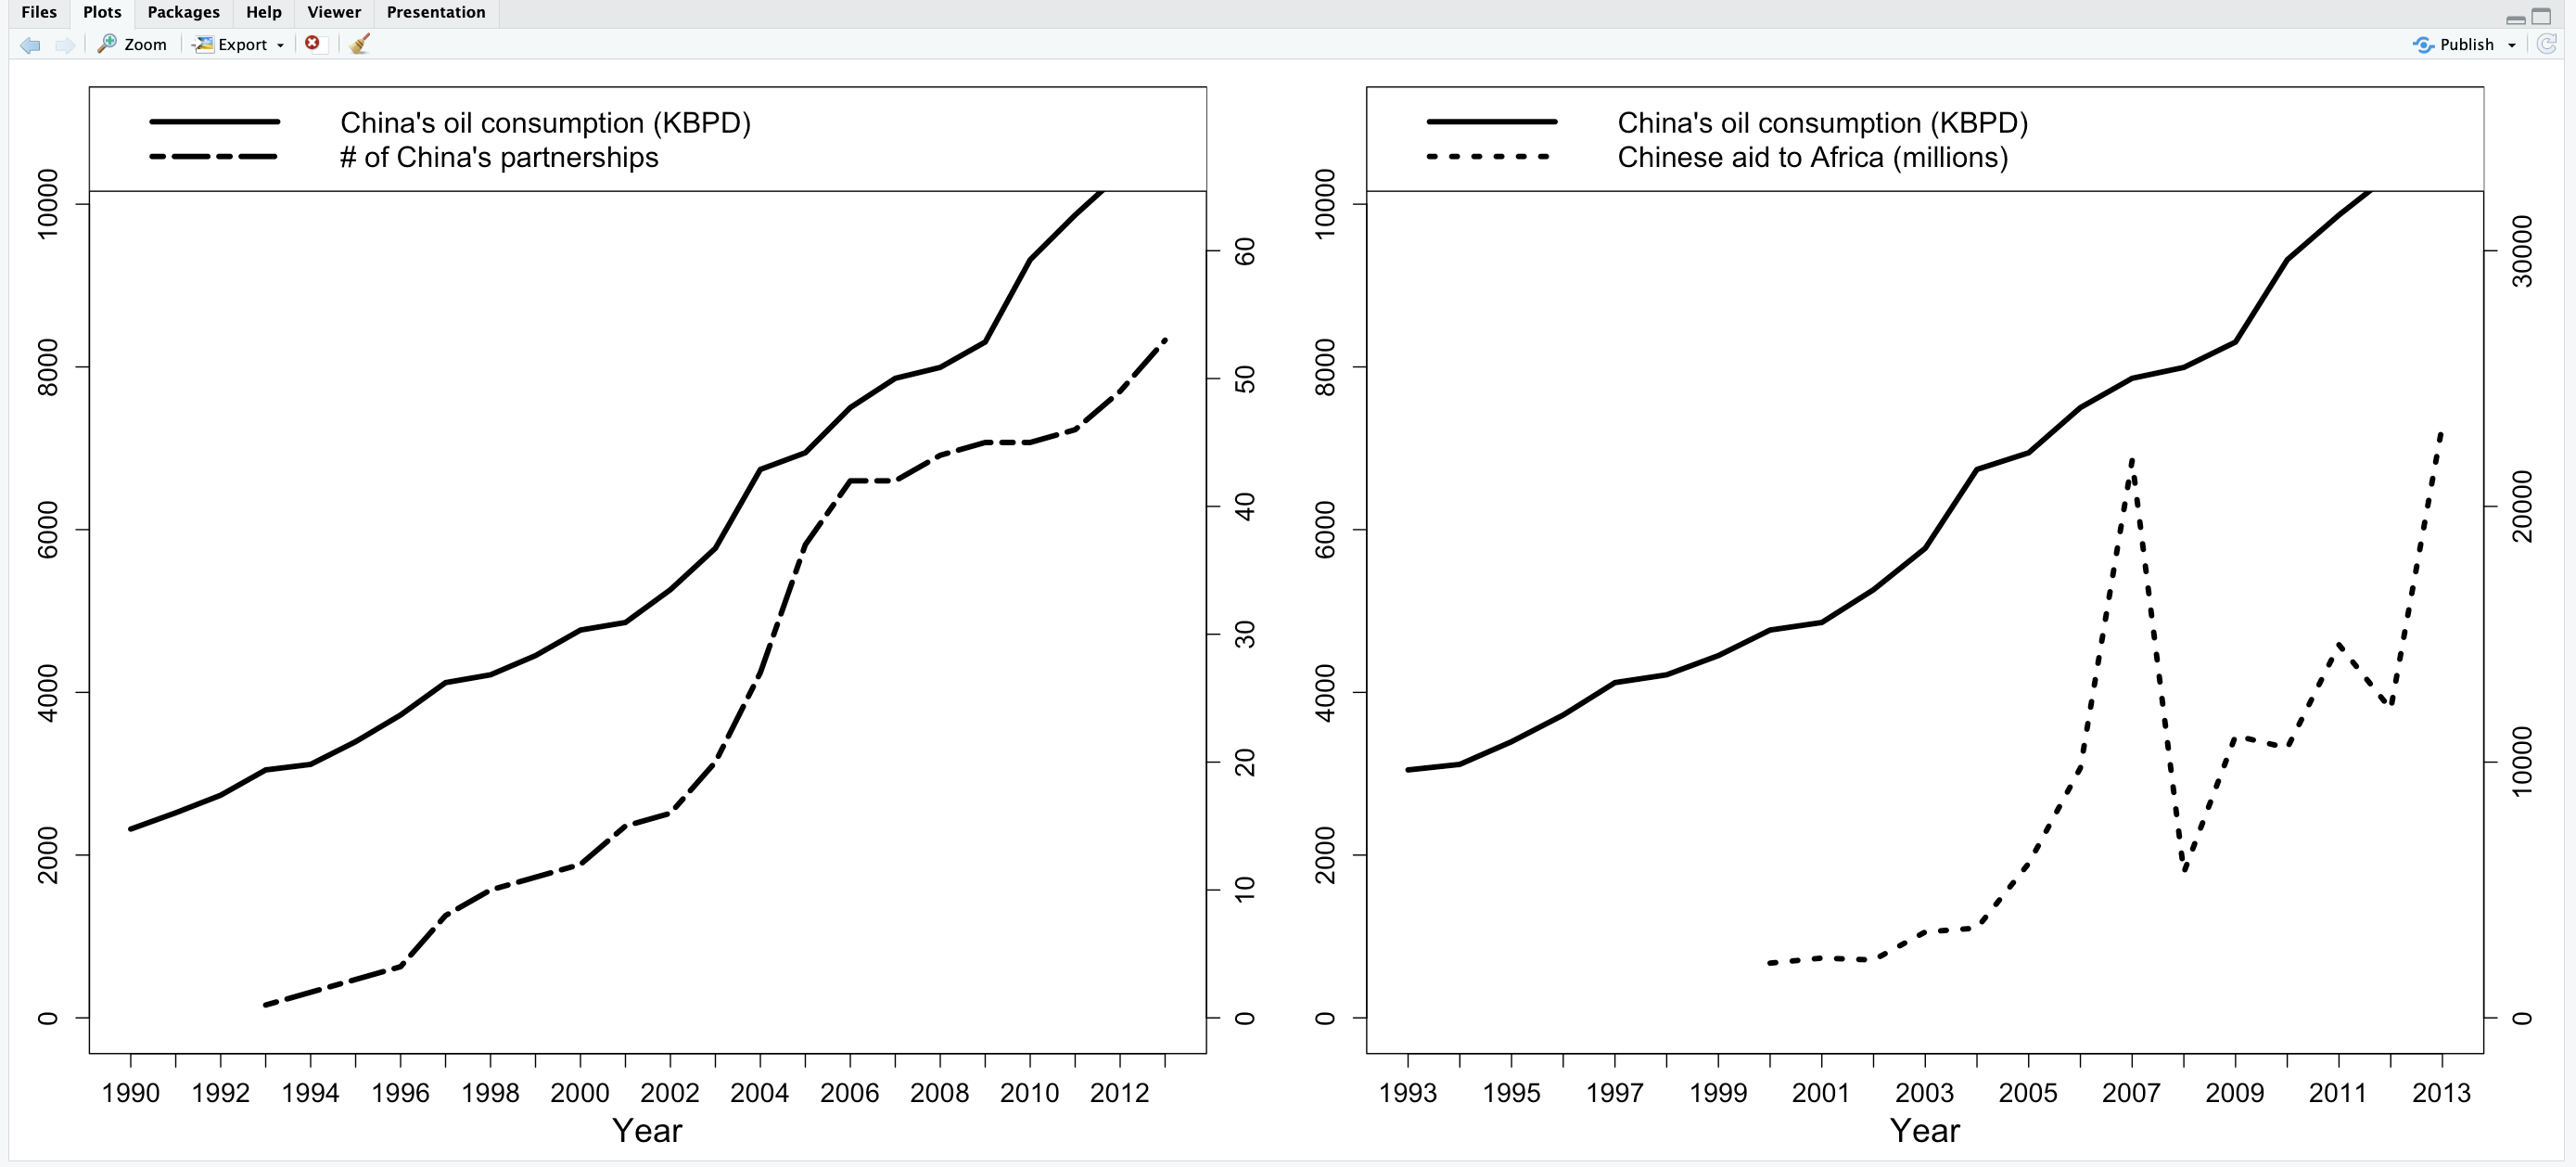
\includegraphics[width=1\linewidth]{figure1r.png}
\end{figure}

\textit{(I chose to include screenshots from R deliberately to show that this is my replication, not a copy-paste of the identical graphical figures from the paper itself...)}


\textbf{Figure 2:}
\lstinputlisting[language=R, firstline=157, lastline=204]{MSChina_energy_Lee_replicate.R} 

\begin{figure}[H]
    \centering
    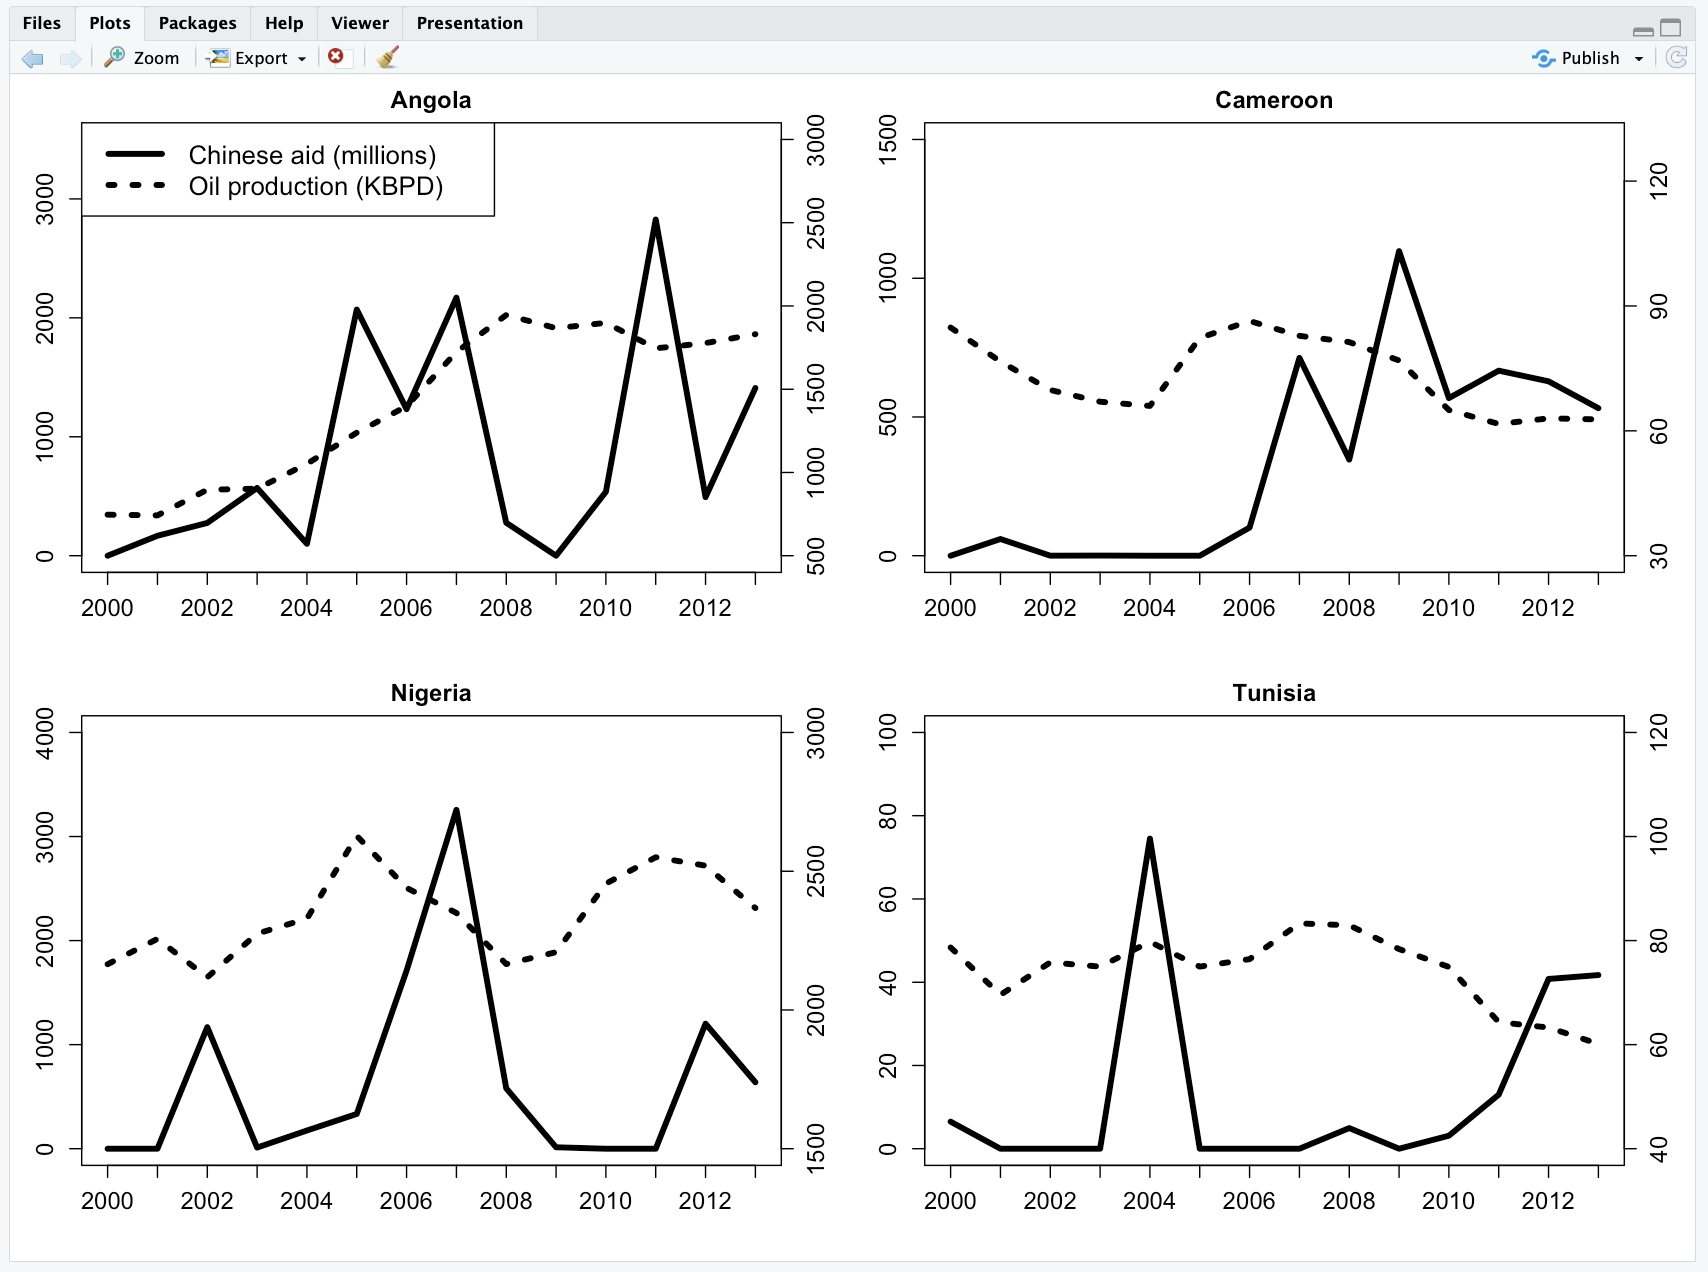
\includegraphics[width=1\linewidth]{figure2r.png}
\end{figure}

\newpage
\section{References}

\noindent Lee, C. (2019). China’s Energy Diplomacy: Does Chinese Foreign Policy Favor Oil-Producing Countries? \textit{Foreign Policy Analysis}, \textbf{15}(4), 570–588. \url{https://doi.org/10.1093/fpa/orz011} \\

\vspace{0.25cm}

\noindent Lee, C. (2023). "Replication data for 'China's Energy Diplomacy: Does Chinese Foreign Policy Favor Oil Producing Countries?'" [Data set]. Harvard Dataverse. \url{https://doi.org/10.7910/DVN/7E3O5P}, V1, UNF:6:x+exuF4WVfknqWQhUWz4MQ== [fileUNF].

\end{document}
